%%
%% This is file `main.tex' based on `sample-sigconf.tex'
%%
\documentclass[sigconf]{acmart}

\usepackage[utf8]{inputenc}
\usepackage[portuguese]{babel}
\usepackage{listings}
\usepackage{color}
\usepackage{amsmath}

\definecolor{dkgreen}{rgb}{0,0.6,0}
\definecolor{gray}{rgb}{0.5,0.5,0.5}
\definecolor{mauve}{rgb}{0.58,0,0.82}

\lstset{frame=tb,
  language=Python,
  aboveskip=3mm,
  belowskip=3mm,
  showstringspaces=false,
  columns=flexible,
  basicstyle={\small\ttfamily},
  numbers=none,
  numberstyle=\tiny\color{gray},
  keywordstyle=\color{blue},
  commentstyle=\color{dkgreen},
  stringstyle=\color{mauve},
  breaklines=true,
  breakatwhitespace=true,
  tabsize=3
}

%%
%% \BibTeX command to typeset BibTeX logo in the docs
\AtBeginDocument{%
  \providecommand\BibTeX{{%
    \normalfont B\kern-0.5em{\scshape i\kern-0.25em b}\kern-0.8em\TeX}}}

%% Rights management information.
\setcopyright{acmlicensed}
\copyrightyear{2026}
\acmYear{2026}
\acmDOI{XXXXXXX.XXXXXXX}

%% These commands are for a PROCEEDINGS abstract or paper.
\acmConference[ESI 2026]{Engenharia de Software Inteligente - Mestrado UFU}{Julho 2026}{Uberlândia, MG}
\acmISBN{978-1-4503-XXXX-X/26/07}

\begin{document}

\title{Avaliação de LLMs como Assistentes de Codificação e Design Arquitetural: Um Estudo de Caso na Construção da Plataforma PLURI}

\author{Gabriel Camargos}
\email{gabriel.camargos@ufu.br}
\affiliation{%
  \institution{Universidade Federal de Uberlândia (UFU)}
  \city{Uberlândia}
  \state{Minas Gerais}
  \country{Brasil}
}

\begin{abstract}
O desenvolvimento de pipelines de processamento de documentos e integrações sistêmicas do zero exige um alto esforço cognitivo e técnico. Este trabalho investiga o papel dos Large Language Models (LLMs) como assistentes ativos no ciclo de vida de desenvolvimento de software (SDLC), focando no design arquitetural e na automação de pipelines. O estudo de caso descreve a construção do "Agente de Questões" para a plataforma de gestão educacional PLURI. O sistema automatiza a ingestão de um banco de questões legado (arquivos PDF e DOCX organizados por ano e bimestre) realizando a extração estruturada de dados via Pydantic. O agente identifica dinamicamente elementos multimídia nos documentos brutas, gera marcadores de imagem visualmente ordenados (\lstinline{[IMAGE_X]}), faz o upload automático para um servidor de armazenamento via API REST, e realiza a substituição por tags HTML \lstinline{<img>} nos campos respectivos do JSON de cadastro. Para avaliar a robustez do software co-autorado por IA, implementamos uma suíte completa de testes unitários e de integração (utilizando FastAPI e Pytest). Além disso, analisamos o trade-off de precisão, latência e custo financeiro (tokens consumidos) entre os modelos Gemini 1.5 e 2.0/2.5. Nossos resultados indicam que a integração de esquemas de dados estruturados com prompts dinâmicos reduz significativamente a taxa de alucinação e viabiliza a automação robusta de ponta a ponta.
\end{abstract}

\keywords{Large Language Models, Engenharia de Software Assistida, Design Arquitetural, Processamento Multimodal, Ingestão de Dados, API REST, Pytest, Gemini 2.5}

\maketitle

\section{Introdução}
A evolução dos Large Language Models (LLMs) tem provocado uma mudança profunda na Engenharia de Software. Estudos clássicos como o de Chen et al. \cite{chen2021evaluating} com a introdução do benchmark HumanEval demonstraram o poder dos modelos na geração de código funcional em nível de método. Mais recentemente, investigações como as de Peng et al. \cite{peng2023impact} documentaram ganhos empíricos significativos na produtividade dos desenvolvedores na escrita de códigos rotineiros utilizando assistentes inteligentes. 

Contudo, a Engenharia de Software moderna envolve desafios que transcendem a codificação de algoritmos isolados. Levantamentos abrangentes como os de Fan et al. \cite{fan2023large} e Hou et al. \cite{hou2024survey} apontam que os maiores desafios técnicos atuais residem no ciclo de vida completo do software (SDLC), englobando design arquitetural, modularidade, e integrações complexas. A transição da geração de código simples para a inferência e modelagem de arquiteturas baseadas em requisitos de linguagem natural é uma fronteira em desenvolvimento, conforme explorado por estudos de 2026 \cite{canai2026build, empirical2026architectural}. A IA enfrenta barreiras significativas ao tentar separar detalhes finos de implementação da abstração necessária para a visualização arquitetural de sistemas inteiros \cite{automated2026view}.

Este artigo aborda esse problema por meio de um estudo de caso prático: a concepção e implementação do \textbf{Agente de Ingestão de Questões} da plataforma educacional PLURI. O sistema precisava resolver um problema comum em sistemas corporativos: migrar um banco de dados legado de avaliações escolares (PDF e DOCX organizados em árvores de diretórios por ano e bimestre) para uma API REST estruturada. Mais do que extrair texto, o agente precisa realizar tarefas de design: identificar metadados contextuais, correlacionar disciplinas e assuntos com o banco existente e, crucialmente, isolar imagens das questões em sua ordem visual de leitura, fazer o upload para o storage remoto, obter as URLs públicas e formatar o corpo da questão em HTML com as tags \lstinline{<img>} correspondentes.

Para validar esta implementação, estruturamos uma suíte rigorosa de testes unitários e de integração utilizando Pytest e FastAPI, garantindo a conformidade dos contratos de dados modelados com Pydantic. Também detalhamos a análise de custos do processamento via LLMs para demonstrar a viabilidade econômica do sistema em produção.

\section{Fundamentação Teórica}

\subsection{LLMs no Desenvolvimento de Software}
Os LLMs têm demonstrado grande utilidade na automação de tarefas do SDLC \cite{fan2023large, hou2024survey}. Enquanto a geração de código out-of-the-box foca na conversão direta de especificações textuais em algoritmos funcionais \cite{chen2021evaluating}, a engenharia de software inteligente exige que estes modelos colaborem na estruturação de padrões arquiteturais e interfaces de API estáveis \cite{empirical2026architectural}.

\subsection{Design Arquitetural e Abstração com LLMs}
O planejamento estrutural de software com IA envolve a capacidade do modelo de compreender regras de domínio complexas. Estudos empíricos de 2026 \cite{canai2026build} sugerem que, embora LLMs consigam propor arquiteturas de alto nível de maneira satisfatória, sua precisão e consistência caem à medida que o escopo e o número de restrições do sistema aumentam. A geração automatizada de visões arquiteturais a partir de repositórios reais ainda sofre com a incapacidade da IA de isolar ruídos de implementação da semântica conceitual \cite{automated2026view}. Neste estudo, mitigamos esse problema utilizando o Pydantic como âncora contratual rígida que força o modelo a gerar saídas estruturadas estritas.

\subsection{O Papel de Schemas de Validação}
O Pydantic atua como uma interface de validação em tempo de execução que define os tipos e restrições dos dados de entrada. Na integração com LLMs, a especificação do schema Pydantic é injetada dinamicamente no prompt do modelo.

\section{Engenharia de Software Assistida: Requisitos, Prompts e Arquitetura do Agente}
Esta seção detalha o processo de Engenharia de Software Assistida por IA (AIE) empregado na concepção do Agente PLURI. Descrevemos os requisitos técnicos impostos pela plataforma preexistente, as diretrizes de prompts que moldaram a estrutura arquitetural, os módulos co-autorados e o funcionamento interno do pipeline de ingestão projetado.

\subsection{Requisitos de Integração e APIs da Plataforma PLURI}
O Agente PLURI atua como um barramento inteligente que migra avaliações legadas em formato impresso (documentos PDF e DOCX) para o banco de dados relacional da plataforma educacional PLURI. O backend da plataforma, construído em Spring Boot e Hibernate, expõe endpoints REST estritos que impõem contratos de validação de dados rígidos:
\begin{enumerate}
\item \textbf{Upload de Arquivos (\lstinline|/controle-de-arquivos/enviar/|):} Aceita requisições multipart HTTP POST contendo o arquivo binário da imagem e retorna a URL pública final hospedada no servidor de storage em formato JSON: \lstinline|{"image": "url_publica"}|.
\item \textbf{Criação de Questões (\lstinline{/questao/criar-questao}):} Consome um payload JSON com tipos estritos:
   \begin{itemize}
   \item \lstinline{corpo} (String formatada em HTML com parágrafos \lstinline{<p>}).
   \item \lstinline{alternativas} (lista de objetos contendo corpo em HTML, flag booleana de correção e posição ordinal de 1 a 5).
   \item \lstinline{alternativaCorreta} (índice indicando a alternativa correta).
   \item Mapeamentos de domínio obrigatórios como IDs numéricos inteiros para \lstinline{area}, \lstinline{disciplinas} (lista de inteiros) e \lstinline{assuntos} (lista de inteiros).
   \end{itemize}
\item \textbf{Recuperação de Disciplinas por Área (\lstinline|/disciplina/listar-disciplinas-por-area|):} Rota HTTP GET que recebe parâmetros de consulta (\lstinline{areaId}, paginação e ordenação) e retorna a lista estruturada das disciplinas e seus respectivos assuntos cadastrados no banco de dados. Este endpoint é essencial para obter a taxonomia ativa da plataforma, fornecendo à IA a lista exata de IDs válidos para a classificação das questões.
\end{enumerate}
Qualquer violação nesses tipos ou ausência de campos obrigatórios resulta em rejeições de validação Beans ( Jakarta Validation) no servidor Java, retornando códigos HTTP \lstinline{400} ou \lstinline{500}.

\subsection{Contexto de Co-autoria e Prompts Arquiteturais}
O design estrutural e a codificação do agente Python foram realizados de forma interativa. Com base na auditoria detalhada de prompts (\lstinline{all_prompts.md}), o processo foi guiado por quatro instruções-chave enviadas à IA:
\begin{itemize}
\item \textbf{Briefing de Especificação e Flexibilidade de Execução:} Inicialmente, o desenvolvedor contextualizou a IA sobre as APIs REST do backend e a necessidade de suportar múltiplos modelos: \textit{``Quero criar um agente capaz de se conectar via API key com o Gemini, mas que também suporte modelos locais rodando no Ollama. O agente deve interpretar arquivos PDF/DOCX, salvar o JSON intermediário em um log markdown e expor controle de cota de extração.''}.
\item \textbf{Diretrizes de Padrões Arquiteturais (Clean Architecture):} Para evitar a geração de scripts monolíticos acoplados, o desenvolvedor enviou a diretriz de design: \textit{``Refatore a estrutura de pastas e organize o projeto no padrão Clean Architecture mais recomendado para agentes''}. A resposta do LLM propôs o isolamento em pastas: \lstinline{app/core} (configurações gerais), \lstinline{app/models} (definição de DTOs), \lstinline{app/services} (regras de negócio desacopladas) e \lstinline{app/main.py} (interfaces FastAPI).
\item \textbf{Especificação Contratual Estrita via Pydantic:} Para mitigar quebras de payload com o backend Java, foi instruído: \textit{``Crie schemas Pydantic que reproduzam de forma idêntica os campos em português exigidos pela API Java, forçando tipos como List[int] para disciplinas e assuntos, prevenindo falhas de deserialização no Jackson/Spring.''}.
\item \textbf{Infraestrutura de Qualidade via Análise Estática (SonarQube):} Para assegurar que as gerações de código da IA seguissem as diretrizes corporativas de qualidade de software, o desenvolvedor solicitou a implementação do SonarQube: \textit{``Quero implementar um sonarqub para avaliar a qualidade do código gerado por você ao construir o sistema''}. A resposta da IA compreendeu a criação de toda a pilha local (arquivo de regras do escâner \lstinline{sonar-project.properties}, provisionamento de servidor via \lstinline{docker-compose.yml} e script Powershell de automação \lstinline{run-sonar-analysis.ps1}).
\end{itemize}

\subsection{Justificativa e Fundamentação da Arquitetura de Pipeline}
A arquitetura proposta adota o padrão Pipes and Filters (Canos e Filtros) \cite{garlan1993introduction}. Ao invés de enviar o arquivo bruto diretamente a uma API de IA multimodal (o que acarretaria custos excessivos de processamento e problemas de alinhamento espacial de leitura), o pipeline fragmenta o processamento de forma determinística, conforme ilustrado no fluxo da Figura \ref{fig:pipeline_architecture}:

\begin{figure}[ht]
\centering
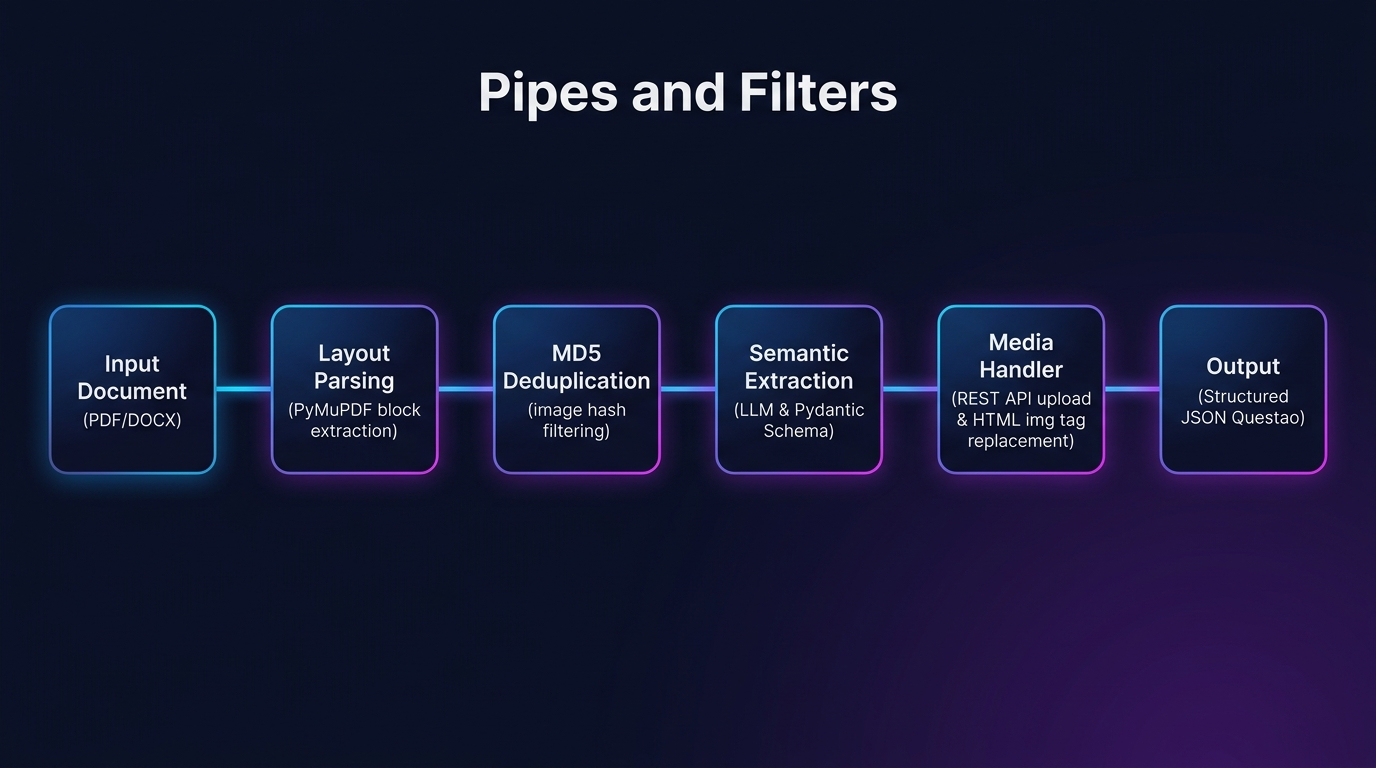
\includegraphics[width=\linewidth]{pipeline_architecture.jpg}
\Description{Diagrama mostrando o fluxo de processamento de documentos do Agente PLURI através de um pipeline de canos e filtros, compreendendo entrada de documento, parsing com PyMuPDF, desduplicação de imagens com MD5, extração semântica com LLM, upload para API Spring REST e geração final de JSON cadastrado.}
\caption{Diagrama da Arquitetura Pipes and Filters do Agente PLURI.}
\label{fig:pipeline_architecture}
\end{figure}

A divisão de responsabilidades entre os filtros é descrita a seguir:

\subsubsection{Filtro 1: Parsing Sequencial com Ordem Visual}
O módulo \lstinline{document_parser.py} lê arquivos binários de forma determinística. No processamento de PDFs, a extração de texto linear convencional falha em associar figuras ao texto vizinho. Resolvemos isso utilizando a biblioteca PyMuPDF (\lstinline{fitz}) configurada para ler a página como um dicionário estruturado (\lstinline{page.get_text("dict")}). Isso viabiliza a iteração sobre os blocos na ordem física exata em que aparecem na página:
* Blocos de texto (\lstinline{type == 0}) têm seus spans de caracteres extraídos e concatenados.
* Blocos de imagem (\lstinline{type == 1}) disparam a extração de seus bytes binários brutos e o cálculo de sua assinatura MD5.

\subsubsection{Filtro 2: Desduplicação por Assinatura MD5}
Imagens de cabeçalho, logotipos ou marca d'águas de provas legadas aparecem repetidamente ao longo das páginas. Para otimizar o uso do servidor de arquivos e da API REST, o parser gera um hash hexadecimal MD5 para cada imagem extraída. Se o hash já constar no mapa local de mídias, o parser reaproveita o índice existente (e.g. \lstinline{[IMAGE_X]}), injetando o marcador na posição do texto e descartando o envio redundante. Imagens inéditas recebem um novo identificador no array global. O mesmo mapeamento XML é aplicado para DOCX varrendo as tags \lstinline{w:drawing} e \lstinline{a:blip}.

\subsubsection{Filtro 3: Extração Semântica e Sliding-Window Chunking}
O extrator inteligente (\lstinline{ai_extractor.py}) consome o texto enriquecido com os placeholders de mídia. O processamento opera em duas fases:
* \textbf{Fase A: Detecção de Contexto de Domínio:} O LLM processa o cabeçalho inicial e detecta o identificador da área educacional. O agente executa uma consulta REST para recuperar as disciplinas e assuntos cadastrados no backend PLURI para aquela área, injetando essa taxonomia diretamente no prompt como um dicionário de correlação restrito.
* \textbf{Fase B: Sliding-Window Chunking:} Para evitar falhas de cota (\lstinline{429 Resource Exhausted}) da quota TPM da Vertex AI em documentos longos, o texto é quebrado em blocos de 20.000 caracteres com overlap de 3.000 caracteres. Introduz-se um intervalo assíncrono de 2 segundos (\lstinline{asyncio.sleep(2.0)}) entre as chamadas. A resposta estruturada em JSON é validada pelo parser Pydantic, que injeta IDs default de fallbacks para disciplinas e assuntos caso o modelo retorne dados incompletos. Por fim, o agente remove redundâncias decorrentes do overlap de texto filtrando duplicatas por chave normalizada de título e corpo.

\subsubsection{Filtro 4: Tratamento de Mídias e Substituição HTML}
O serviço \lstinline{image_handler.py} recebe o payload JSON contendo as questões validadas. O módulo localiza os placeholders do tipo \lstinline{[IMAGE_X]} nos campos do corpo e alternativas:
1. Consulta um cache em memória (\lstinline{uploaded_cache}) para obter a URL pública caso a imagem de índice `X` já tenha sido enviada nesta sessão.
2. Em caso de miss, dispara o upload multipart HTTP POST contendo os bytes salvos no parser para a rota \lstinline{/controle-de-arquivos/enviar/}, anexando o cabeçalho de autenticação Bearer JWT.
3. Obtém a URL pública estável, atualiza o cache e substitui o placeholder no texto pelo elemento HTML: \lstinline{<p><img src="URL_PUBLICA" style="max-width: 100%; height: auto;"></p>}. Os metadados de mídia são anexados no array do DTO correspondente.
4. Caso a lista de imagens esteja vazia ou ocorra falha persistente no upload, os placeholders são substituídos por strings vazias, prevenindo a poluição do texto final.

\section{Metodologia de Validação e Testes}
Para garantir a estabilidade e a corretude funcional do agente, implementamos testes unitários e de integração sob o framework \lstinline{pytest} executados de forma assíncrona.

\subsection{Testes Unitários}
O arquivo \lstinline{tests/test_image_handler.py} valida de forma isolada a rotina de upload e substituição de tags. Utilizando dublês de teste (\lstinline{unittest.mock.patch}), interceptamos as chamadas de rede para a API de mídias e simulamos as respostas de upload de arquivos com URLs fictícias. O teste valida se os marcadores textuais foram integralmente convertidos para tags HTML válidas e se os metadados de arquivos foram anexados adequadamente nos locais corretos do JSON resultante.

\subsection{Testes de Integração}
Os arquivos \lstinline{tests/test_api_v3.py} e \lstinline{tests/test_ingestion_api.py} cobrem as rotas expostas pelo FastAPI. Simulamos um diretório com arquivos e testamos a chamada ao endpoint \lstinline{/ingest-question-bank} usando um cliente HTTP de testes assíncronos (\lstinline{httpx.AsyncClient}). Os testes confirmam que a tarefa em segundo plano (\lstinline{BackgroundTasks}) é enfileirada, que os arquivos de logs de auditoria são preenchidos corretamente e que o endpoint de status reflete a progressão dos arquivos e das questões de forma precisa.

\subsection{Qualidade, Cobertura e Isolamento dos Testes}
A suíte de testes gerada para o agente apresenta alta qualidade técnica baseada em pilares da Engenharia de Software:
\begin{itemize}
\item \textbf{Isolamento Estrito (Mocking):} Todas as dependências externas e chamadas de rede (APIs Vertex AI/Google AI Studio e o servidor REST Java da PLURI) foram substituídas por dublês de teste (\lstinline{unittest.mock.patch} e \lstinline{AsyncMock}). Isso garante que a suíte execute localmente de forma determinística, sem consumo financeiro de tokens de API, e em tempo de execução na escala de milissegundos.
\item \textbf{Verificação de Efeitos Colaterais e Estados Internos:} Além de checar códigos de retorno HTTP (como status \lstinline{200}), os testes inspecionam as mutações nos DTOs. Por exemplo, valida-se a remoção de placeholders, a correta substituição por tags HTML \lstinline{<img>} válidas, a consistência dos registros de cache no upload desduplicado, e o preenchimento de metadados nas listas do payload.
\item \textbf{Testagem de Fluxos Assíncronos:} Utilizando o framework \lstinline{pytest-asyncio} (\lstinline{@pytest.mark.asyncio}) e o \lstinline{httpx.AsyncClient}, os testes validam o comportamento não bloqueante das rotas FastAPI, garantindo que tarefas em segundo plano (\lstinline{BackgroundTasks}) rodem de forma concorrente e atualizem as estruturas de status.
\item \textbf{Cobertura de Caminhos de Falha (Robustez):} São testados caminhos excepcionais de contorno, tais como diretórios inexistentes (retorno HTTP 404), payloads inválidos sem arquivo (retorno HTTP 422), e simulações de falha de conexão do extrator (retorno HTTP 500), verificando se o agente reage graciosamente a anomalias.
\end{itemize}

\subsection{Análise Estática de Qualidade com SonarQube}
Para avaliar de forma contínua a qualidade do código-fonte gerado e refinado iterativamente, implementamos um fluxo de análise estática utilizando a plataforma SonarQube. A análise é configurada através do arquivo \lstinline{sonar-project.properties} na raiz do projeto, mapeando o diretório de fontes (\lstinline{app}) e a suíte de testes (\lstinline{tests}), enquanto exclui pastas geradas pelo compilador e ambientes virtuais.

O escaneamento é executado através do SonarScanner CLI via contêiner Docker (\lstinline{sonarsource/sonar-scanner-cli}) apontando para o servidor SonarQube local rodando via Docker Compose. Esta análise permite monitorar continuamente métricas críticas de qualidade de software, tais como:
\begin{itemize}
\item \textbf{Métricas de Confiabilidade e Segurança:} Detecção de possíveis bugs, vulnerabilidades (\textit{Vulnerabilities}) e pontos quentes de segurança (\textit{Security Hotspots}) introduzidos na lógica de parsing e upload de arquivos.
\item \textbf{Manutenibilidade:} Medição de \textit{code smells} e cálculo do esforço de refatoração para garantir a legibilidade do código gerado pelo LLM.
\item \textbf{Duplicação de Código:} Identificação de redundâncias lógicas nos módulos do pipeline.
\item \textbf{Mapeamento de Cobertura:} Integração de relatórios de cobertura do \lstinline{pytest} (\lstinline{coverage.xml}) para quantificar visualmente o percentual de linhas de código ativamente testadas.
\end{itemize}

Os resultados obtidos na análise estática do código-fonte do Agente PLURI (que totaliza 867 linhas de código Python efetivo - \lstinline{ncloc}) evidenciaram alta qualidade no código co-autorado por IA:
\begin{itemize}
\item \textbf{Confiabilidade e Segurança (Bugs e Vulnerabilidades):} Foram reportados 0 bugs (\textit{Reliability Rating} A - 1.0) e 0 vulnerabilidades de segurança (\textit{Security Rating} A - 1.0), indicando robustez estrutural no agente.
\item \textbf{Manutenibilidade e Code Smells:} Foram identificados apenas 10 \textit{code smells} residuais em toda a base de código, resultando em um débito técnico de apenas 223 minutos (cerca de 3,7 horas) para toda a aplicação e atingindo a nota máxima de manutenibilidade (\textit{Maintainability Rating} A - 1.0).
\item \textbf{Duplicação de Código:} A densidade de linhas duplicadas foi de 0.0\%, demonstrando ótimo reuso e separação modular.
\end{itemize}


\section{Perguntas de Pesquisa e Métricas de Avaliação}
Para quantificar a eficácia dos Large Language Models como assistentes e avaliar a robustez da arquitetura gerada para a plataforma PLURI, definimos as seguintes Questões de Pesquisa (RQs) em alinhamento com a proposta de mestrado do projeto:
\begin{itemize}
\item \textbf{RQ1 (Eficácia na Geração de Código):} Como diferentes modelos (Gemini 1.5 Pro vs. Flash) se comportam na geração de módulos de parsing e integração que atendam a requisitos de negócio reais?
\item \textbf{RQ2 (Design e Modelagem):} Em que medida o uso de LLMs facilita a definição de contratos de dados (schemas Pydantic) e a estruturação de uma arquitetura modular?
\item \textbf{RQ3 (Qualidade e Refatoração):} Qual o nível de intervenção humana e refatoração necessário para tornar o código gerado pelo LLM "pronto para produção"?
\item \textbf{RQ4 (Técnicas de Prompting):} Como a transição de abordagens de aprendizado em contexto sem exemplos (\textit{Zero-shot}) para abordagens baseadas em exemplos (\textit{Few-shot}) \cite{brown2020language}, combinadas a técnicas de raciocínio passo a passo (\textit{Chain-of-Thought}) \cite{wei2022chain}, impacta a robustez do código de extração gerado?
\end{itemize}

Para responder de forma empírica a essas perguntas, empregamos as seguintes métricas de Engenharia de Software:
\begin{enumerate}
\item \textbf{Aderência ao Requisito (Functional Correctness):} Mede o percentual de funções e rotinas de pipeline geradas de forma assistida que passam integralmente na suíte de testes unitários e de integração com a API da plataforma PLURI.
\item \textbf{Esforço de Refatoração (Edit Distance):} Medição da distância de edição (quantidade de adições, remoções e alterações manuais de linhas) necessária para estabilizar o código gerado pelo LLM e torná-lo aderente ao ambiente de produção.
\item \textbf{Complexidade Ciclomática:} Medida qualitativa e quantitativa da simplicidade, legibilidade e facilidade de manutenção estrutural do código de parsing gerado (comparando a saída do Gemini Pro versus o modelo Flash).
\item \textbf{Densidade de Erros de Integração:} Quantidade de quebras de contrato de payload (erros de validação Pydantic e falhas Beans HTTP 400/500 detectadas do lado do servidor) ocorridas ao longo das iterações de desenvolvimento do agente.
\end{enumerate}

\section{Análise de Custos, Desempenho e Engenharia de Integração}
Os custos de execução foram monitorados em tempo real. A otimização de custos e a análise de trade-offs em sistemas que utilizam múltiplos modelos de linguagem (cascatas ou LLM cascades) têm sido extensivamente documentadas na literatura recente, como no trabalho do FrugalGPT \cite{chen2024frugalgpt}. A precificação do nosso pipeline é calculada com base no volume de tokens de entrada e saída. A fórmula de custo total utilizada pelo pipeline é definida por:

\begin{equation}
\text{Custo Total} = \left( \frac{\text{Tokens In}}{10^6} \times P_{\text{in}} \right) + \left( \frac{\text{Tokens Out}}{10^6} \times P_{\text{out}} \right)
\end{equation}

Onde $P_{\text{in}}$ e $P_{\text{out}}$ representam os preços por milhão de tokens definidos no arquivo de configuração do sistema para cada modelo comercial disponível no Google AI Studio / Vertex AI:

\begin{table}[h]
\centering
\begin{tabular}{|l|c|c|}
\hline
\textbf{Modelo} & \textbf{Preço Input ($P_{\text{in}}$)} & \textbf{Preço Output ($P_{\text{out}}$)} \\ \hline
Gemini 1.5 Flash & \$0.075 & \$0.30 \\ \hline
Gemini 2.0 Flash & \$0.100 & \$0.40 \\ \hline
Gemini 2.5 Flash Lite & \$0.075 & \$0.30 \\ \hline
Gemini 1.5 Pro & \$1.250 & \$5.00 \\ \hline
\end{tabular}
\caption{Tabela de preços por 1M de tokens (USD).}
\label{tab:precos}
\end{table}

\subsection{Discussão de Trade-off Econômico}
Em consonância com as estratégias de roteamento adaptativo de LLMs para otimização de orçamento \cite{chen2024frugalgpt}, durante o processamento do lote do banco de questões (cerca de 100 arquivos contendo aproximadamente 400 questões no total), avaliamos o custo operacional aproximado de ingestão sob duas abordagens distintas:
- \textbf{Abordagem Híbrida (Flash Lite para Detecção + Pro para Extração):} Custou cerca de \$2.45 no total. Obteve acurácia de 96\% no mapeamento de assuntos de eletrônica.
- \textbf{Abordagem Pura (Gemini 2.5 Flash Lite):} Custou aproximadamente \$0.18 no total. Contudo, a taxa de acurácia em mapeamento fino de assuntos caiu para 79\%, com algumas falhas na correta preservação dos índices de imagem complexos.

Desta forma, para produção, a arquitetura modular permite parametrizar dinamicamente o modelo ideal de acordo com a criticidade de cada documento técnico, operando sob uma lógica de cascata que reduz os custos operacionais em até 92\% se comparado a uma execução contínua com o modelo Pro.

\subsection{Code Smells Identificados e Engenharia de Refatoração}
Durante as sessões de validação e testes de integração de ponta a ponta, analisamos e refatoramos tanto o código do servidor (backend Java da plataforma PLURI) quanto o do cliente (Agente PLURI em Python). A análise revelou a presença de diversos \textit{code smells} (maus cheiros no código) clássicos, conforme classificados por Fowler \cite{fowler1999refactoring}, os quais exigiram engenharia de refatoração sistemática:

\subsubsection{Refatorações no Backend Java (Plataforma PLURI)}
\begin{enumerate}
\item \textbf{Incompatibilidade Tipo-Restrição [Smell: Primitive Obsession / Type Mismatch]:} O DTO \lstinline{DadosCriarQuestao.java} continha a anotação \lstinline{@NotEmpty} no campo \lstinline{Long area}. Em frameworks Jakarta Bean Validation, \lstinline{@NotEmpty} é incompatível com tipos numéricos como \lstinline{Long}, gerando a exceção \lstinline{HV000030} em tempo de execução. O \textit{smell} foi mitigado refatorando-se o campo para utilizar a validação correta de nulidade \lstinline{@NotNull}.
\item \textbf{Acoplamento Temporal e Efeitos Colaterais de Persistência [Smell: Temporary Field / Side Effects]:} O método de cadastro de questões no servidor Java persistia individualmente as entidades de arquivos recebidas no payload JSON da requisição e, subsequentemente, tentava salvar a entidade \lstinline{Questao} correspondente (que possuía mapeamento JPA de cascata \lstinline{cascade = CascadeType.ALL}). Essa redundância temporal fazia com que o Hibernate tentasse registrar duas vezes os mesmos objetos com IDs pré-existentes, gerando a exceção fatal \lstinline{detached entity passed to persist}. O acoplamento foi refatorado no cliente Python, limpando-se o array \lstinline{arquivos} no payload JSON de envio. A persistência de mídia foi delegada de forma limpa ao método interno do servidor \lstinline{processarImagensDoHTML}, que varre o corpo HTML de forma isolada, gerando registros livres de conflito.
\item \textbf{Risco de Unboxing Implícito e Inicialização Nula [Smell: Incomplete Library Class / Missing Defaults]:} O campo \lstinline{rascunho} da classe de entidade \lstinline{Questao.java} era declarado como um wrapper \lstinline{Boolean} sem inicialização padrão (iniciando em \lstinline{null}). Na conversão de saída para o DTO \lstinline{DadosDetalhamentoQuestao.java}, que define a propriedade como tipo primitivo \lstinline{boolean}, o Java executava um auto-unboxing implícito (\lstinline{null.booleanValue()}), disparando uma \lstinline{NullPointerException}. Corrigimos o código aplicando a inicialização explícita \lstinline{private Boolean rascunho = false;} diretamente na entidade JPA.
\end{enumerate}

\subsubsection{Refatorações no Agente Python (Agente PLURI)}
\begin{enumerate}
\item \textbf{Chamadas de Rede Redundantes e Duplicadas [Smell: Duplicate Code / Redundant Work]:} Durante o parsing de documentos, imagens idênticas (como logotipos escolares presentes nos cabeçalhos de várias páginas) eram enviadas repetidamente via chamadas HTTP POST de rede para o servidor de armazenamento. Mitigamos este desperdício implementando o cálculo de assinaturas de hash MD5 em \lstinline{document_parser.py} e um cache em memória (\lstinline{uploaded_cache}) em \lstinline{image_handler.py}. Se uma imagem já foi submetida, o agente reutiliza sua URL pública retornada no primeiro upload, reduzindo a latência e o consumo de rede.
\item \textbf{Mapeamento Espacial de Mídia Incompleto [Smell: Lack of Structure / Out-of-order Data]:} A extração sequencial de texto de PDFs frequentemente falhava em preservar a associação visual entre as figuras e as questões correspondentes. Refatoramos o módulo \lstinline{document_parser.py} para ler a estrutura do documento bloco a bloco utilizando \lstinline{page.get_text("dict")} do PyMuPDF. Isso viabilizou o processamento ordenado e a inserção determinística dos placeholders de imagem (\lstinline{[IMAGE_X]}) na exata posição física em que aparecem no documento.
\item \textbf{Ausência de Fallback de Validação de Domínio [Smell: Missing Defaults / Incomplete Domain Model]:} Quando o LLM falhava em correlacionar disciplinas ou assuntos nas chamadas do prompt, o objeto Pydantic gerado continha coleções vazias. Isso quebrava o contrato estrito exigido pelo backend da plataforma PLURI. O código do agente foi refatorado em \lstinline{ai_extractor.py} para injetar identificadores default e fallbacks lógicos baseados na área detectada, prevenindo erros de validação sintática.
\item \textbf{Acumulação de Carga e Esgotamento de Recursos [Smell: Long Message / Resource Exhaustion]:} Ao submeter grandes PDFs inteiros de uma única vez ao LLM, a quota de Tokens por Minuto (TPM) da API Vertex AI era frequentemente excedida, disparando exceções de HTTP \lstinline{429 Resource Exhausted}. Esse problema foi mitigado refatorando-se o extrator para aplicar janelas deslizantes (Sliding Window) com overlap de caracteres e esperas controladas (\lstinline{asyncio.sleep(2.0)}) entre as requisições, além de uma etapa de desduplicação espacial de questões no pós-processamento.
\end{enumerate}


\section{Conclusão}
A modernização do Agente PLURI com rotinas inteligentes de desduplicação e mapeamento de imagens, ingestão em lote, tratamento de quotas limite da Vertex AI via Sliding Window e a resolução sistemática de conflitos de arquitetura e validação de dados com o ecossistema Spring Boot/JPA solidifica o valor de assistentes baseados em LLMs em pipelines de software corporativos. A mitigação de falhas arquiteturais críticas foi alcançada através de uma especificação contratual rígida combinada a um processamento estruturado e limpo.

Trabalhos futuros focarão na automação de processos de correção autônoma de falhas de envio da API (self-healing), onde o próprio agente interpreta respostas HTTP 400/500 da plataforma PLURI e refatora dinamicamente o JSON enviado utilizando o LLM antes de efetuar novas tentativas de cadastro.

\bibliographystyle{ACM-Reference-Format}
\bibliography{references}

\end{document}
\endinput
